\documentclass[11pt,a4paper]{article}
\usepackage{hyperref}


\usepackage{times}
\usepackage[T1]{fontenc}
\usepackage{graphicx}
\usepackage{subfigure}
\usepackage{epsfig}
\usepackage{fancyhdr}
\usepackage[dvipsnames]{color}


\usepackage{courier} % Import the Courier font package

% Define a new command for some words
\newcommand{\retis}{\texttt{reticulate }}
\newcommand{\panels}{\texttt{panelification }}
\newcommand{\reti}{\texttt{reticulate}}
\newcommand{\panel}{\texttt{panelification}}
\newcommand{\harps}{\texttt{harp }}
\newcommand{\harpss}{\texttt{harpSpatial }}

\textwidth = 170.0mm
\textheight = 246.0mm

\topskip=5mm
\topmargin=0mm
\evensidemargin=-5.4mm
\oddsidemargin=-5.4mm
\headheight=14pt
\headsep=5mm

\parindent=0mm
\parskip  =2mm

\pagestyle{fancy}

\fancyfoot[C]{}

\voffset=-1.25cm
%\pagenumbering{arabic}
%\setcounter{page}{1}
\headheight=15pt

%\definecolor{mygray}{cmyk}{0,0,0,0.4}
\definecolor{mygray}{gray}{0.5}
\fancyhf{}
\rhead{\textcolor{mygray}{\fontsize{10}{12}\selectfont F1. Name1, F2. Name2}}
\renewcommand{\headrule}{{\color{mygray}%
       \hrule width\headwidth height\headrulewidth \vskip-\headrulewidth}
}%renewcommand headrule

\renewcommand\textfraction{.02}
\renewcommand\floatpagefraction{.98}

% for rule under section heading
\newcommand {\sectionrule}{\vskip -0.9 cm
\color {mygray} \rule [0 cm] {17 cm}{0.1 mm} \color {black}}

%%%%%%%%%%%%% START %%%%%%%%%%%%% 
\date{}

%\title{Developments done during Polly Schmederer's ACCORD VS at DMI (June 2024) }
\title{Report on a scientific visit on spatial methods with \harps and the \panels tool}

\author{Polly Schmederer (GeoSphere) \\ Carlos Peralta (DMI) \\ Fabrizio Baordo (DMI)}
\date{August 2024}


\begin{document}
\maketitle
\thispagestyle{fancy}
%\begin{flushleft}

\section{Introduction}
\sectionrule
A Visiting scientist (VS) from GeoSphere (Polly Schmederer) visited DMI during June 2024. The VS 
was funded by the ACCORD-VS program, as part of the MQA working package. The VS was hosted by Fabrizio Baordo
and Carlos Peralta at the DMI headquarters in Copenhagen. The 4 weeks stay was focused on the 
implementation  of new capabilities of the \panels tool \cite{panel_tool} developed at GeoSphere to include additional scores and variables. 
Additionally, the use of the \retis package \cite{reticulate}, that provides an interface to the python language from the R language, was also considered.
The whole development is shared in a github repository that includes installation instructions and example data sets \cite{repo}.

A detailed description of the code developments is presented below, along with application examples and future work.

%Generalising spatial verifications: 
%\begin{itemize}
%    \item improving R scripting in 
%    \item use of the \retis package to interface R with Python;
%    \item generalise/apply the \panels tool
%    \item providing examples.
%\end{itemize}

\section{Methods and software used}
The \harps package is a framework for meteorological data developed by Andrew Singleton (Met Norway) and Alex Decknym (RMS) \cite{harp}.
It is currently the official model verification tool in the ACCORD consortium.
The \panels tool is a visualization framework developed at GeoSphere in order to display summarized views of spatial verification scores
produced by the \harpss part of the \harps package \cite{panel_tool}.
The developments during the VS included the extension of new variables in the panel tool and the inclusion of the \retis package in the 
tool chain. 
The \retis package provides an interface between R and the Python language.
This allowed us to easily include some of the vast functionalities available
in Python, for example through the library \texttt{xarray}. This facilitated
the reading and regridding of the input data from satellite (nat format)
and model data from different sources in grib and netcdf format.
%This facilitated the ingestion of new data types in netcdf and grib format.

The general aims of the visit were the following.
\begin{itemize}
    \item Integrate the \panels tool in the \harps library.
    \item Use of the \retis package to interface R with Python;
    \item Generalise/apply the \panels tool to different applications
    \item Providing examples.
\end{itemize}

All the developments were carried out in a branch of the \texttt{oper-harp-verif} repository \cite{oper-harp}.
The \texttt{renv} package was used to create a local R environment where all
the necessary libraries and dependencies can be installed.

\section{Developments in the \panels too and \harpss}

%\sectionrule
%\subsection{Reading functions}

A detailed description of the functions can be found in the \texttt{README.md} file
in the github repository. 
%The functions inside $reading_functions.R$ contains the following reading functions.
%\begin{itemize}
%\item $$read_msg_reticulate$$  Python function that reads/ regrids the data and converts the returned data into a harp data frame.
%\item $$read_nc_reticulate$$ calls python function that reads snow data and converts the returned data into a harp data frame.
%\item $$reading_functions.py$$ Contains the python functions that are called by R to read / regrid satellite observations ( in .nat format ) and model data (.grib).
%\item $$sat_model_to_same_grid$$ reads/ regrids satellite data.
%\item $$get_data_nc_file()$$ reads regridded snow data in nc format.
%\end{itemize}
%\subsection{Panelification}
%\subsection{Configuration files}
%\subsection{Installation instructions}
\section{Data used for spatial verification}

%The headings of main sections are underlined. This is achieved by the new command "sectionrule".


%An example of a Table is given in \ref{tab:grib}. Please feel free to make a more fancy one if you like.
A list of the different types of input data used in the examples can be found in table \ref{tab:grib}. %Please feel free to make a more fancy one if you like.

\begin{table}
{\center\it\caption{ \label{tab:grib} Input data}}
\begin{center}
\begin{tabular}{lrr}
 Model                                       & DINI & DEODE \\
 Parameter    &   tot prec & tot prec \\
 %Type of level (Code Table 3).          &   105  &   1 \\
 %Time unit (Code Table 4).              &     1  &   1 \\
 %Time range one.                        &     0  &   6 \\
 %Time range two.                        &     6  &   0 \\
 %Time range indicator (Code Table 5)    &     4  &   0 \\
\end{tabular}
\end{center}
\end{table} 

\section{Application examples}


%\begin{figure}[ht] %[h*]
%\begin{center}
% \centerline{
%   \figure{file=../PLOTS/panel_IR_108_202401022300+23.png,scale=0.6}
%  }
%\end{center}

\begin{figure}[htbp]
    \centering
    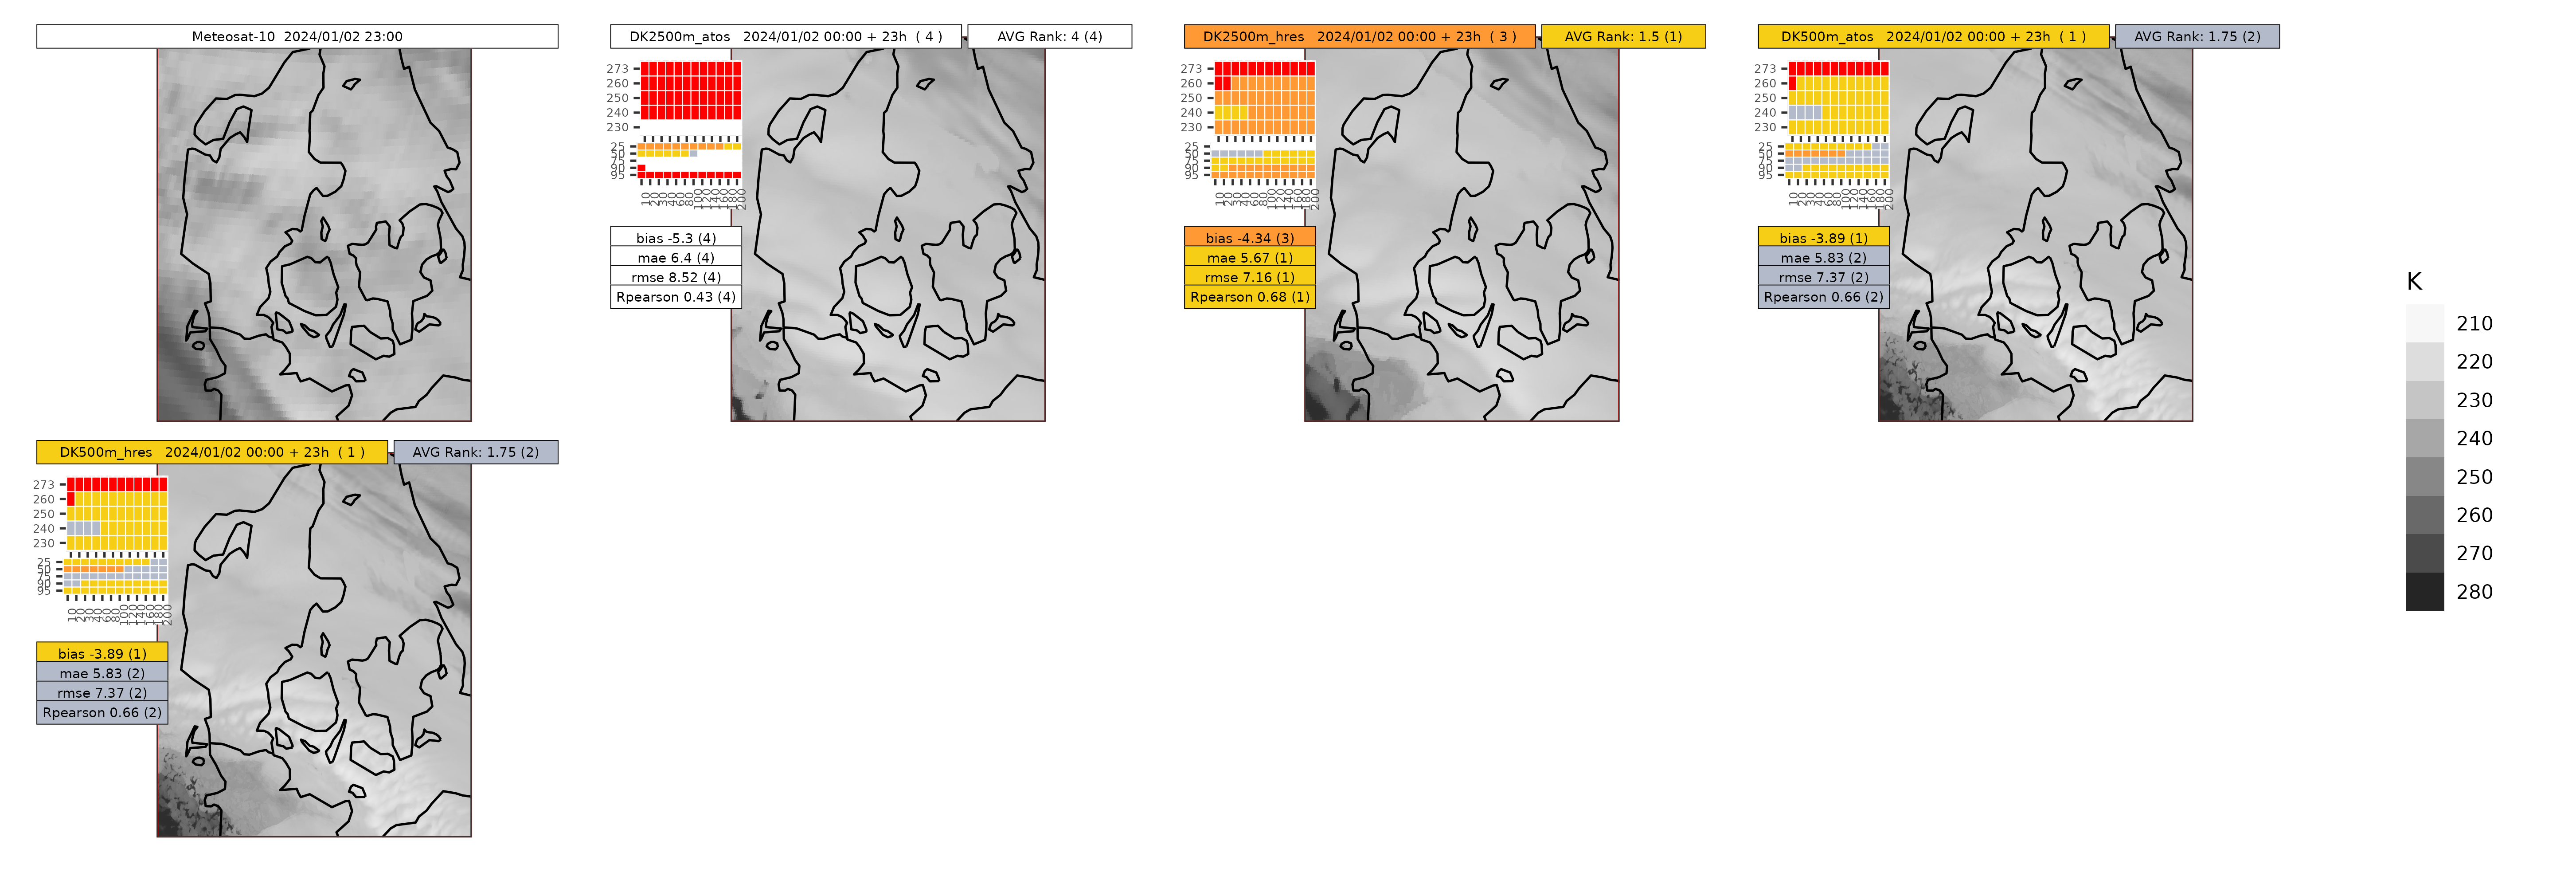
\includegraphics[width=1.2\textwidth]{../PLOTS/panel_IR_108_202401022300+23}
    \caption{EUMETSAT SEVIRI data}
    \label{fig:IRexample}
\end{figure}

\begin{figure}[htbp]
    \centering
    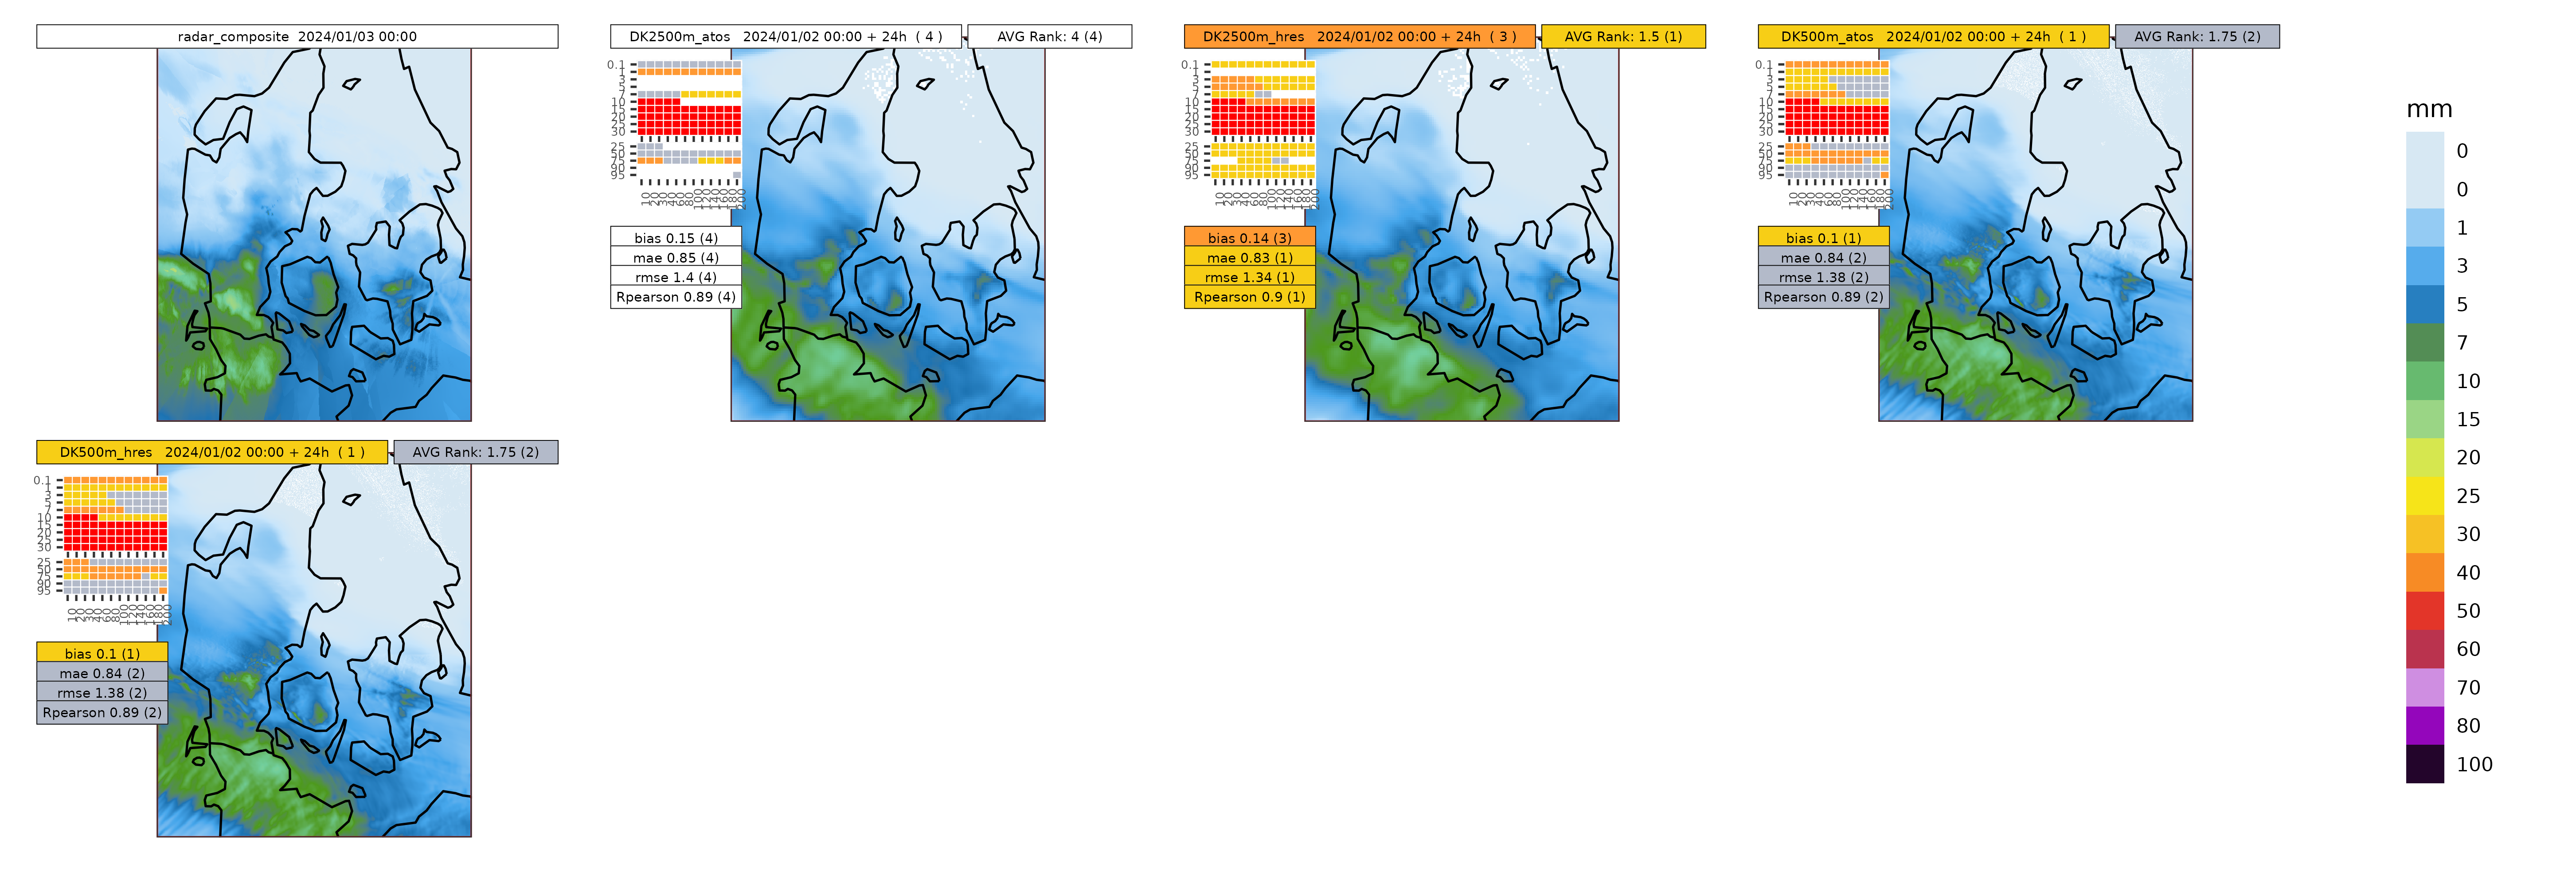
\includegraphics[width=1.2\textwidth]{../PLOTS/panel_Accpcp3h_202401030000+24.png}
    \caption{DMI radar data}
    \label{fig:TPexample1}
\end{figure}
%  {\center\it\caption{\label{fig:O3}
%   Title of my figure}}
%\end{figure}
%\subsection{Figure layout}
%Figures have to be provided in high resolution, preferably in Encapulated PostScript (eps) format, or ".png", ".jpg" or ".gif". 
%\textbf{Please, NO .PS files (PDFLaTeX cannot use .ps image files to produce a .pdf file).}
%In principle it is best to provide me seperately the image files that are closest to the creating source and have not yet been converted into another format.
%
%The picture caption is placed under the picture, in italic, for example see Figure \ref{fig:O3}.
%
%Please be careful with the size of your picture. LibreOffice has tools to reduce the size of the .pdf file created from your article (with reducing the definition of the pictures). It's not the case with latex (or I don't know how to do that), thus the pictures you provide should have reasonable size.
%
%\begin{figure}[ht] %[h*]
%\begin{center}
%  \centerline{
%   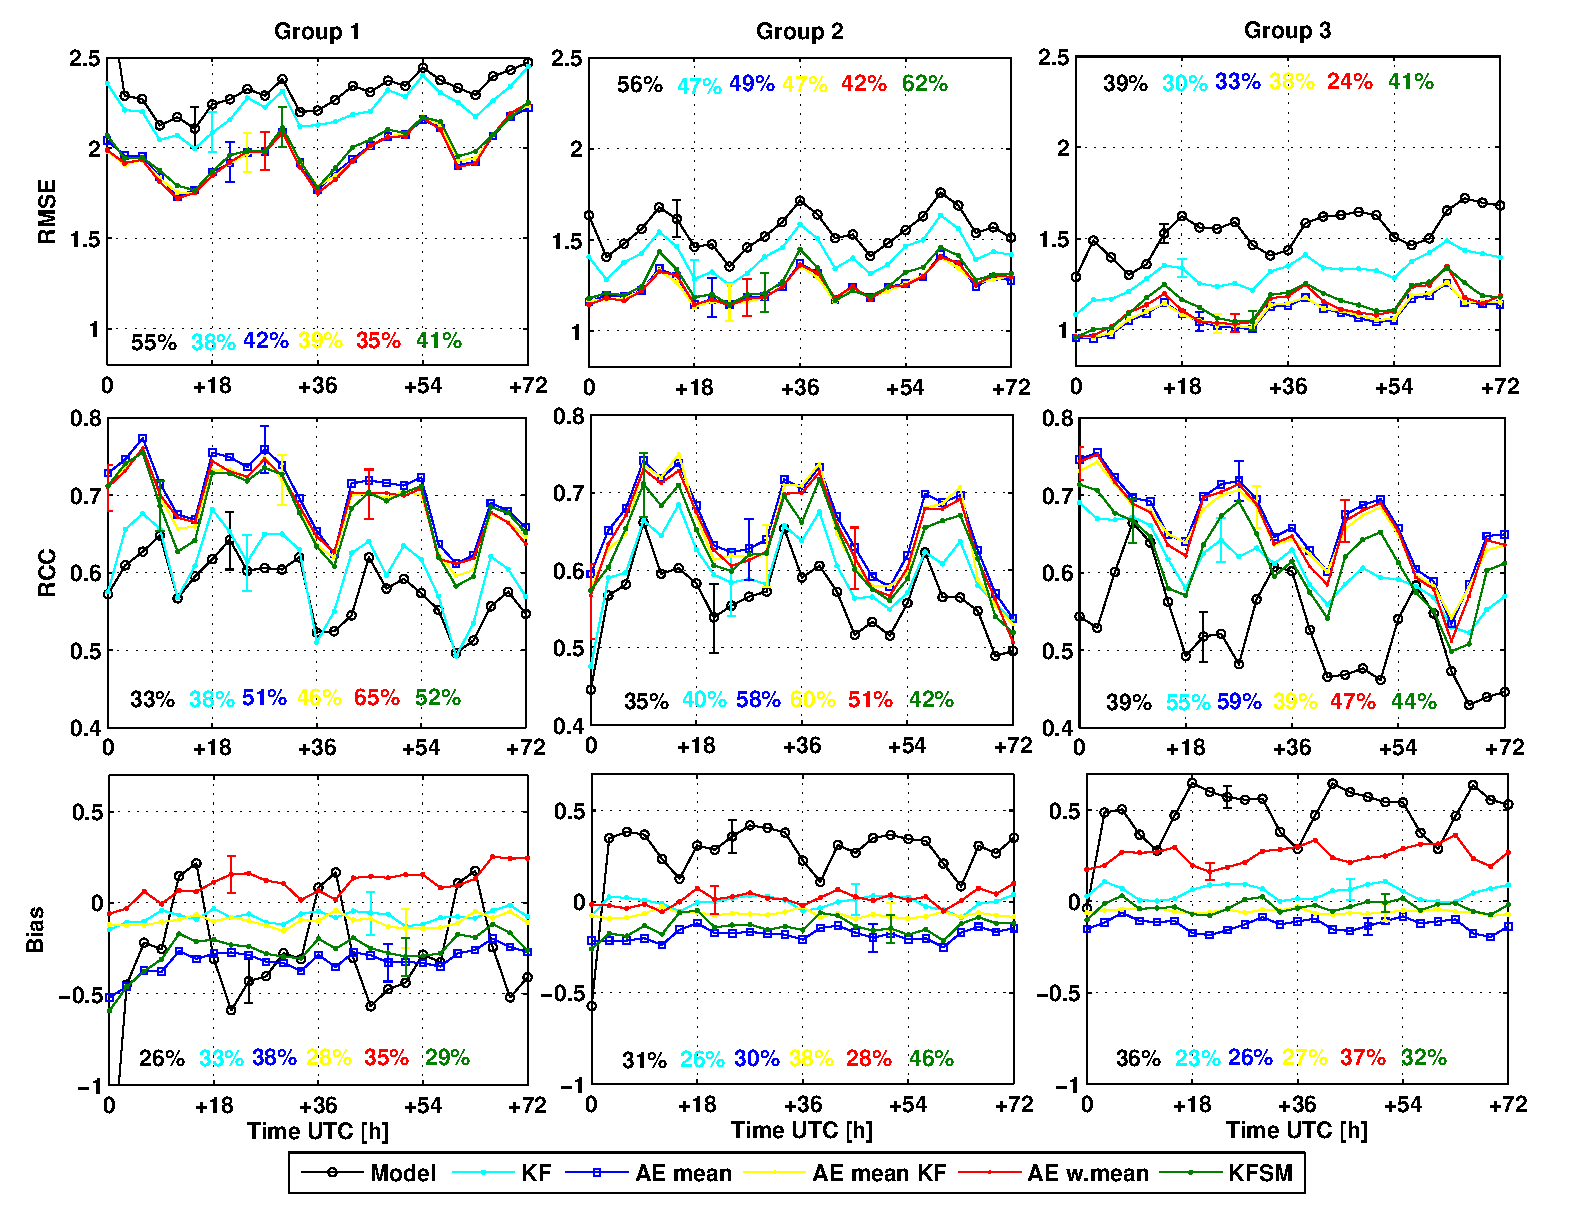
\epsfig{file=./exemple.eps,scale=0.6}
%  }
%\end{center}
%  {\center\it\caption{\label{fig:O3}
%   Title of my figure}}
%\end{figure}

\section{Future work}


%\section{References}

\bibliographystyle{plain}
\bibliography{references}


%\end{flushleft}
\end{document}

 
